% ------------------------------------------------------------------------
% -*-TeX-*- -*-Hard-*- Smart Wrapping
% ------------------------------------------------------------------------
\def\baselinestretch{1}

\chapter{Results}

\def\baselinestretch{1.44}

%%% ----------------------------------------------------------------------
The Results section offers a thorough overview of the conclusions drawn from our methodology, with a special emphasis on the ability of the Random Forest model to forecast changes in the price of bitcoin.

\smallskip

%%% ----------------------------------------------------------------------
\goodbreak
\section{Random Forest Performance}
\goodbreak

A well-known ensemble learning technique called Random Forest combines predictions from various decision trees to provide a consolidated result. It is a great tool for predicting Bitcoin values due to its complex capacity to unravel non-linear patterns in datasets.


\subsection{Model Training and Validation:}

Time Series Cross-Validation (TSCV) was used to train and validate the model. This method is specifically designed for time series data, such as Bitcoin price data, where the sequential nature of data points is crucial. The model was tested over five different training-validation windows to guarantee robustness.

A Multiple Training Windows Approach was also used to investigate the effect of training window size on model performance. The size of the training window can be quite important. More historical data is available with a bigger training window, which may help to identify long-term trends. A smaller window, though, might be more responsive to current developments. The model was trained using three different lengths of historical data: 50 percent, 60 percent, and 70 percent of the dataset, in order to determine the best window size for our data.

\subsection{Performance Metrics across Validation Windows:}

-	\textbf{Root Mean Squared Error (RMSE): }

\begin{figure}[H]
\centering
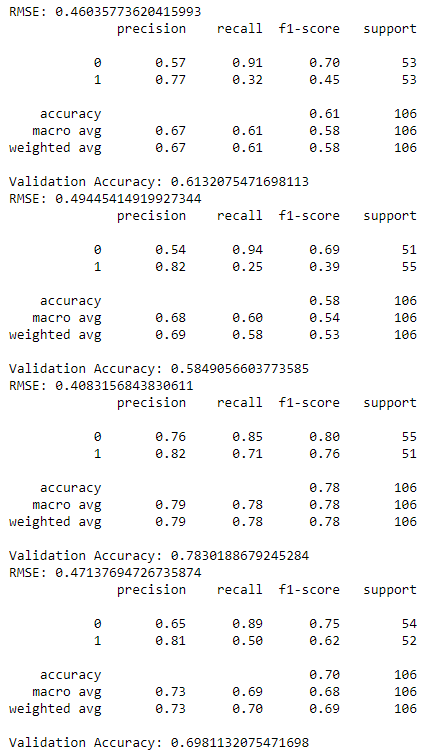
\includegraphics[scale=0.85]{fig2.jpg}
\end{figure}

\begin{figure}[H]
\centering
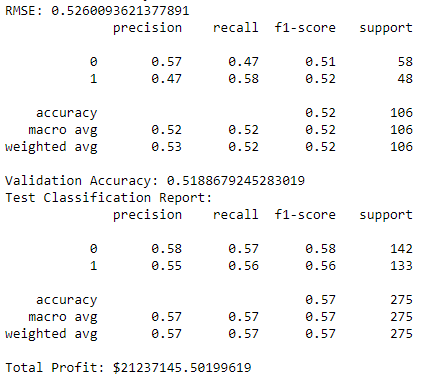
\includegraphics[scale=0.85]{fig3.jpg}
\end{figure}

RMSE is a metric for gauging how well a model predicts a result. Lower RMSE values are preferred since they show better data fit. The observed RMSE values were 0.460, 0.494, 0.408, 0.471, and 0.526 for the five validation windows. The variation in RMSE across windows highlights the underlying volatility of Bitcoin values.

-	\textbf{Accuracy:} The ratio of successfully predicted instances to all instances is provided by this metric. Across the five validation windows, the model received accuracy scores of 61.32 percent, 58.49 percent, 78.30 percent, 69.81 percent,51.89 percent, and 57.00 percent, respectively. Given the unpredictability of cryptocurrency prices, these figures suggest a fair amount of fit.

-	\textbf{Precision:} Represents the proportion of accurate positive forecasts among all positive predictions. Precision for estimating price increase (1) ranged from 0.82 to 0.47 among the from 0 to 1 window.

-	\textbf{Recall:} Indicates the proportion of accurate positive forecasts among all real positives. The range of recall values for forecasting price increases was 0.25 to 0.94 among the 0 to 1 window.

-	\textbf{F1 Score:} The harmonic mean of recall and precision is the F1-score. A balanced performance was shown by F1-Scores for predicting price increases, which varied from 0.39 to 0.80 among the 0 to 1 window.


\medskip

\textbf{Performance in the Multiple Training Windows Approach Across Different Windows:}

\begin{figure}[H]
\centering
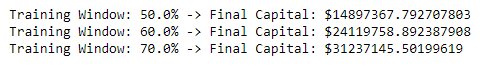
\includegraphics[scale=0.85]{fig4.jpg}
\end{figure}

-	\textbf{Training Window 50 percent:} Using half the dataset for training produced a final capital of about 14,897,367.79 Dollars, indicating a 4,897,367.79-dollar profit from an initial 10,000,000 Dollars.

-	\textbf{Training Window 60 percent:} The model technique resulted in a capital of about 24,119,758.89 Dollars, indicating a profit of about 14,119,758.89 Dollars, with a training window of 60 percent of the dataset.

-	\textbf{Training Window 70 percent:}  70 percent of the data was used for training, producing a capital of around 31,237,145.50 Dollars and a profit of about 21,237,145.50 Dollars.



\subsection{Visualization insights:}

Three useful visualizations were produced:

\textbf{1. Predicted Return Probabilities Over Time:} 

\begin{figure}[H]
\centering
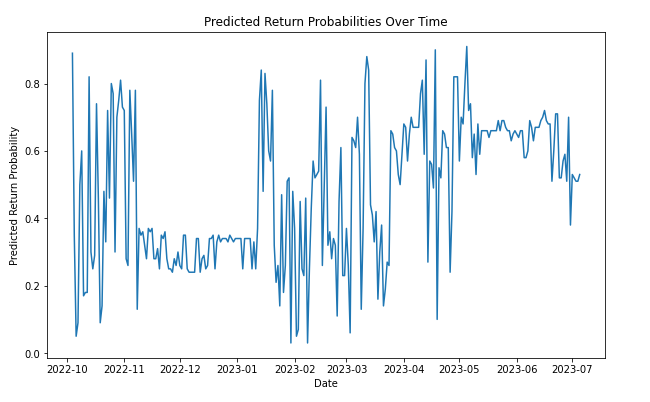
\includegraphics[scale=0.85]{fig5.jpg}
\caption{Predicted Return Probabilities Over Time}
\label{Predicted Return Probabilities Over Time}
\end{figure}

Figure 4.1 shows how expected return probabilities fluctuated during the test period.

This graph illustrates how confidently the model makes predictions over time. A higher probability denotes a more fervent expectation that the price will increase the following day.

\textbf{2.	Cumulative Profit/Loss Over Time:}

\begin{figure}[H]
\centering
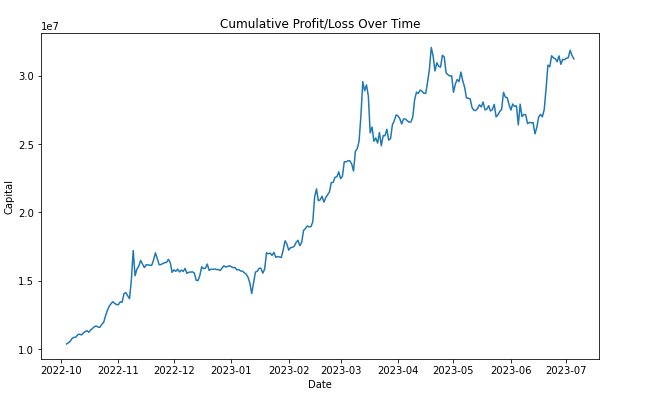
\includegraphics[scale=0.85]{fig6.jpg}
\caption{Cumulative Profit/Loss Over Time}
\label{Cumulative Profit/Loss Over Time}
\end{figure}

Figure 4.2 shows the cumulative profit/loss trajectory when using the trading suggestions from the algorithm.

This visualization illustrates the overall financial effects of using the trading strategy suggested by the model. The profitability of the strategy is indicated by a steadily increasing trend.

\textbf{3.	Final Capital vs. Training Window Size:} 


\begin{figure}[H]
\centering
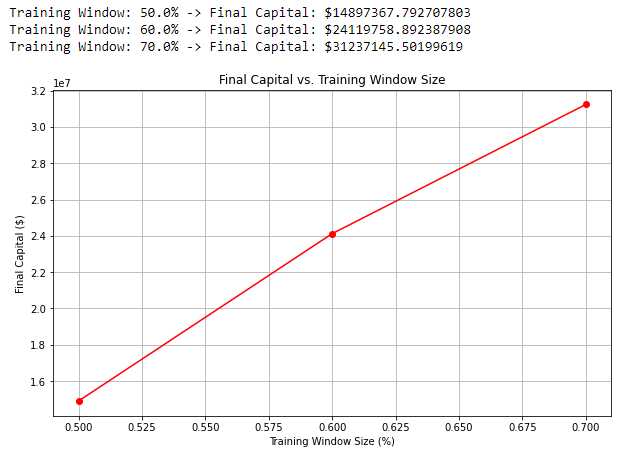
\includegraphics[scale=0.85]{fig7.jpg}
\caption{Final Capital vs. Training Window Size}
\label{Final Capital vs. Training Window Size}
\end{figure}
Figure 4.3 shows the connection between the dimensions of the training windows and the total capital gained. As seen, greater earnings result from a wider training window.

A plot juxtaposing the final capitals against the training window sizes was generated for a clearer understanding.

\subsection{Comparison of trading Strategies(Long or Cash)(Long or Short) In Random Forest}

\textbf{Model Performance: }
During cross-validation, the model's performance on several validation sets is presented. The model's accuracy, sensitivity, and harmonic mean of precision and recall are revealed through metrics like precision, recall, and f1-score.

\textbf{Results of a trading strategy:}

\textbf{Long or Cash Strategy}: With 10 million dollars in initial capital, the strategy generates a profit of about 13.21 million Dollars.

\textbf{Long or Short Strategy}: This strategy generates a higher profit of about 21.24 million dollars using the same initial cash.

\textbf{Visualization: }

A plot depicts the overall profit or loss for both techniques over time. Understanding the capital's growth trajectory and contrasting the performance of the two strategies over the test set is made easier thanks to this graphical representation.

\begin{figure}[H]
\centering
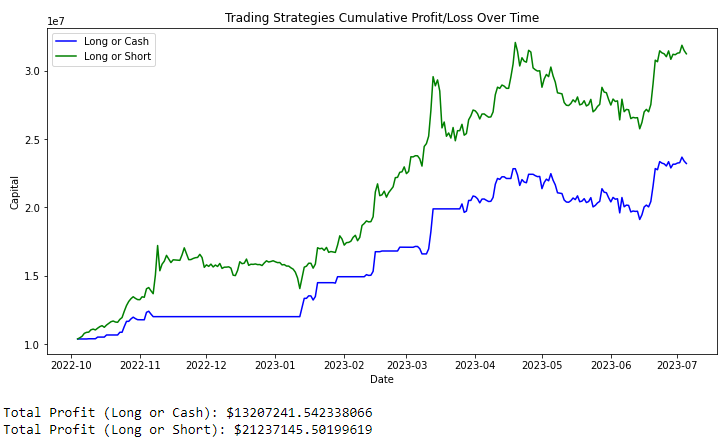
\includegraphics[scale=0.85]{fig8.jpg}
\caption{Comparison of trading Strategies(Long or Cash)(Long or Short) }
\label{Comparison of trading Strategies(Long or Cash)(Long or Short)}
\end{figure}

\subsection{Conclusion for Random Forest Performance:}

A few significant findings are shown when the Time Series Cross-Validation (TSCV) and Multiple Training Windows techniques:

\textbf{Model Robustness:} The Random Forest model produced profits consistently over a range of validation windows and training sizes.
Optimal Window Size: The best window size produced a profit of 70 percent, indicating that using more historical data can help project Bitcoin values.

\textbf{Economic Significance:} In addition to traditional performance measurements, the significant profits made highlight the model's useful applications for Bitcoin trading. Understanding the practical ramifications of these forecasts is essential in addition to the measurements. An overall profit of 21,237,145.50 Dollars was realized by applying a straightforward trading strategy based on the model's predictions on the validation set. This large number highlights the usefulness and potential profitability of utilizing the Random Forest model to anticipate Bitcoin trade.

\goodbreak
\section{LSTM Performance}
\goodbreak

Recurrent neural network (RNN) architecture's Long Short-Term Memory (LSTM) networks, a subtype, are lauded for their aptitude for identifying and understanding long sequences. Due to its suitability for time series forecasting, which calls for the detection of patterns in sequential data \citep{Hochreiter1997LongSM}. 

\subsection{Model Training and Validation:}

\textbf{Model Architecture:}

The LSTM model's architecture consisted of two LSTM layers, followed by a Dense layer. To guarantee sequential input for the following LSTM layer, the first 50 units of the LSTM layer were programmed to return sequences. It was intended for the terminal Dense layer to produce a single value that foretells the following data point in the series. The model used the Adam optimizer for optimization and Mean Squared Error as the loss function.

\textbf{Training Across Multiple Windows:}

Temporal patterns are frequently visible in financial data, especially time series data. To determine the ideal window size for prediction, the LSTM model in this study was trained on historical data spanning window sizes of 60 percent, 70 percent, 80 percent, and 90 percent of the training data.

\subsection{Performance Metrics Across Training Windows:}

\textbf{Model Training Iterations:} For optimization, each training window underwent several iterations. The step progress bar (example: [================ Depending on the size of the window, each iteration took different amounts of time; larger windows took longer because there was more data to process. For illustration:

60 percent of the training window was finished in 8 iterations.
70 percent of the training window was finished in 6 iterations.
80 percent of the training window was finished in 4 iterations.
90 percent of the training window was finished in 2 iterations.

\textbf{Trading Strategy: }

Following the prediction, a "long or short" trading strategy was implemented. A long position (asset purchase) was taken if the model indicated an upward trend (rising price). Conversely, a short position was taken (asset sold) if a downward movement (price drop) was anticipated.

\textbf{Test Set Evaluation: }

The model was retrained on the entire training set after identifying the ideal training window size, and it was then assessed on a different test set. After applying the "long or short" trading method to the test data, the total portfolio value was roughly 19,002,979.05 Dollars. This implies that, when used in trading, the forecasts of the LSTM model may yield large profits. Given an original investment of 10,000,000.00 Dollars, this predicts a profit of about 9,002,979.05 Dollars.

\subsection{Visualization Insights: }
Plotting the actual vs. expected Bitcoin prices was shown in a visualization. The model's capacity to forecast over time is shown visually, enabling a qualitative evaluation of the model's accuracy and dependability.


\begin{figure}[H]
\centering
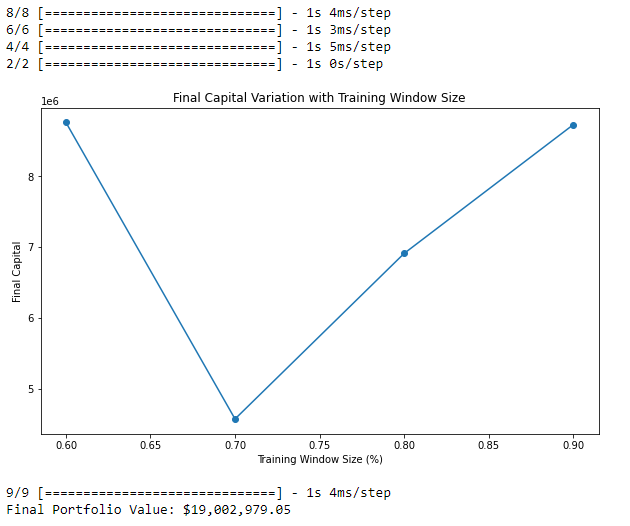
\includegraphics[scale=0.85]{fig9.jpg}
\caption{Final Capital Variation with Training Window Size}
\label{Final Capital Variation with Training Window Size}
\end{figure}

Figure 4.5: A graphic illustration showing how the size of the training window and the resulting final capital relate to one another. Notably, bigger training windows appeared to bring in more money.

The actual vs forecasted Bitcoin values over time were displayed in a different visualization, which sheds light on the model's predictive power and the efficacy of the "long or short" trading approach:



\begin{figure}[H]
\centering
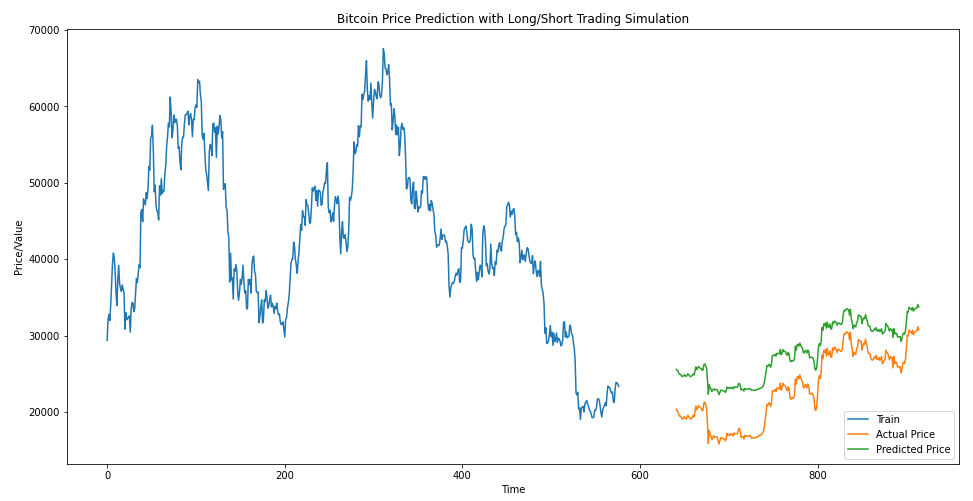
\includegraphics[scale=0.65]{fig10.jpg}
\caption{Bitcoin Price Prediction with Long/Short Trading Simulation }
\label{Bitcoin Price Prediction with Long/Short Trading Simulation }
\end{figure}

Figure 4.6 shows a comparison graph between the model's predictions and the actual prices of Bitcoin. Understanding the model's adherence to actual price movements is made easier thanks to this visualization.

\subsection{LSTM Model With Adjusted (No of Days)}

\begin{enumerate}
    \item \textbf{Import Necessary Libraries:}
\end{enumerate}

Libraries for managing data (numpy and pandas), preparing data (MinMaxScaler), creating models (keras LSTM model), and visualizing data (matplotlib) are all imported.

\textbf{2. Data Loading and Preprocessing:}

A data frame called df is filled with Bitcoin price information.

Datetime formatting is applied to the Date column.

The date is used to order the data.

The daily \% change in closing prices is calculated and stored in a new column called Return.

\textbf{3. Data Normalization:}

Only the Close prices—which are kept in new data—are taken into account for modeling.

The closing prices are then normalized (scaled) with MinMaxScaler, a typical preprocessing step for neural networks so that they lie between 0 and 1.

 \textbf{4. LSTM Model Definition:}
To create an LSTM model, a function called create lstm model() is defined. A Dense layer with one unit (for price prediction) follows two LSTM layers with 50 units each in the model.
The model is optimized with the Adam optimizer and utilizes mean squared error as its loss function.

\textbf{5. Splitting the training data:}

The training data is chosen over num days, a predetermined number of days. The remaining data is taken into account for validation.
X train (training) and X valid (validation) sets of the data have been created.

\textbf{6. Model Education:}

With a batch size of 1, the LSTM model is trained on the training data (X train) for 10 epochs.

\textbf{7. Making Predictions}

On the validation data (X valid), predictions are made using the trained LSTM model.
The inverse transformation of MinMaxScaler is then used to change these scaled forecasts back to the original pricing scale.

\textbf{8. Trading Strategy Implementation}

It uses a "long or short" trading approach. A long position is taken (i.e., the model predicts the price will climb) if the forecasted price for the following day is higher than the closing price of the current day. A short position is taken (i.e., the model forecasts the price will decline) if the projection is lower.

Based on the actual price change the following day, the capital is modified. If the price rises, the capital for a long position rises, and if the price falls, the capital for a short position rises.



\textbf{9. Visual Representation:} 

- To show the performance of the model, a graphical representation is made.

- The actual closing prices, the anticipated prices, and the data set intended for training are shown in the graph.

- The effectiveness of the trading technique and the model's alignment of forecast with real price are both revealed by this visualization. 

We can edit the No of days as shown in the figure below and the output will be generated with the portfolio value 

\begin{figure}[H]
\centering
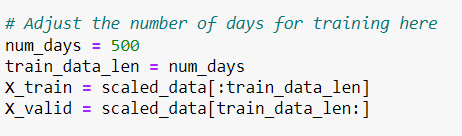
\includegraphics[scale=0.65]{fig15.jpg}
\end{figure}

Below Visualisation is selected in 14 days.

\begin{figure}[H]
\centering
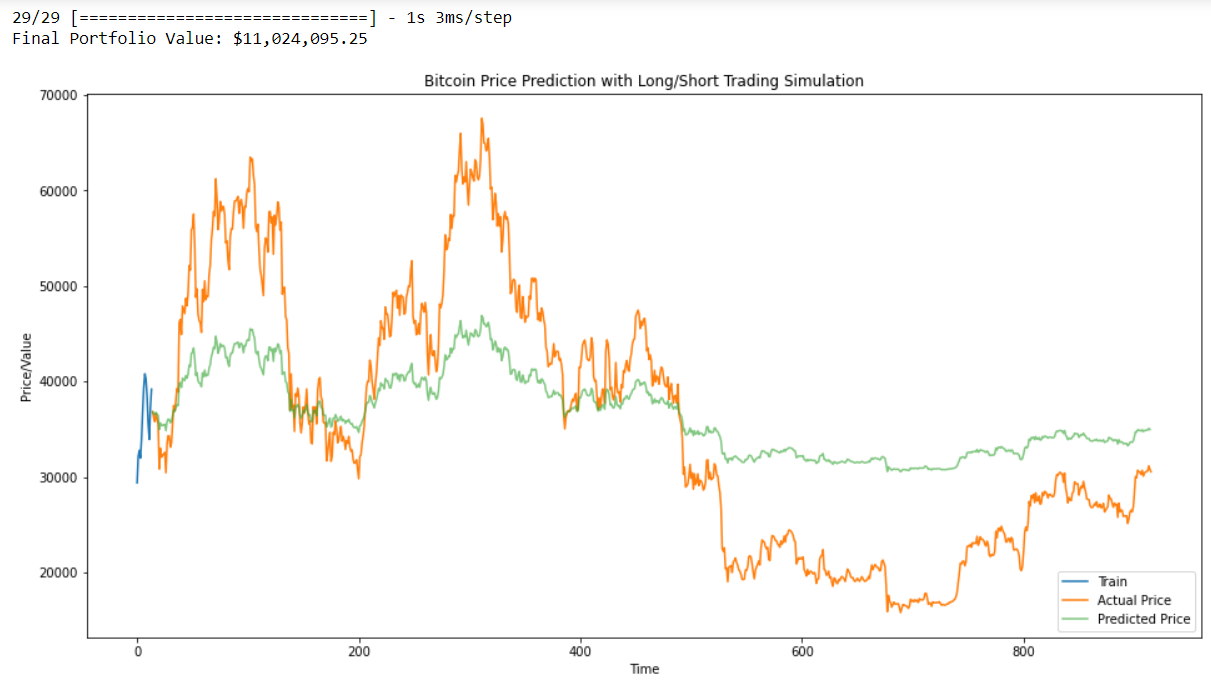
\includegraphics[scale=0.65]{fig11.jpg}
\caption{Adjust the number of days for training(14 Days)}
\label{Adjust the number of days for training}
\end{figure}

Below Visualisation is selected in 30 days.

\begin{figure}[H]
\centering
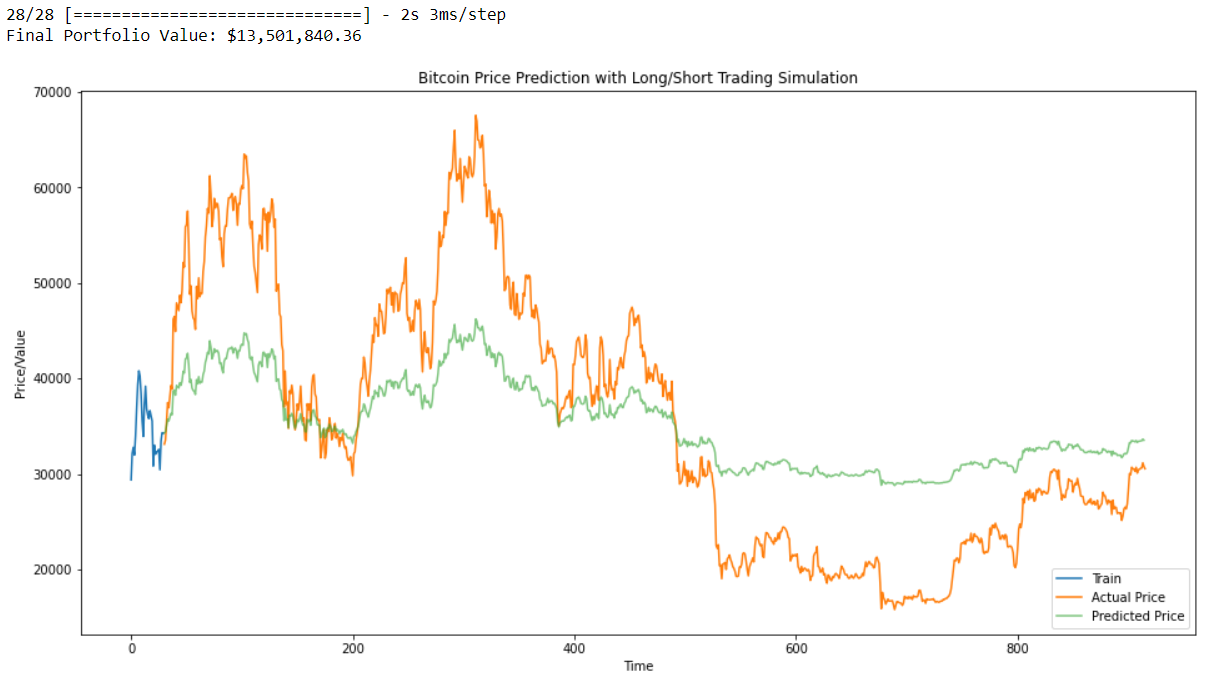
\includegraphics[scale=0.65]{fig12.jpg}
\caption{Adjust the number of days for training(30 Days)}
\label{Adjust the number of days for training}
\end{figure}

Below Visualisation is selected in 90 days.

\begin{figure}[H]
\centering
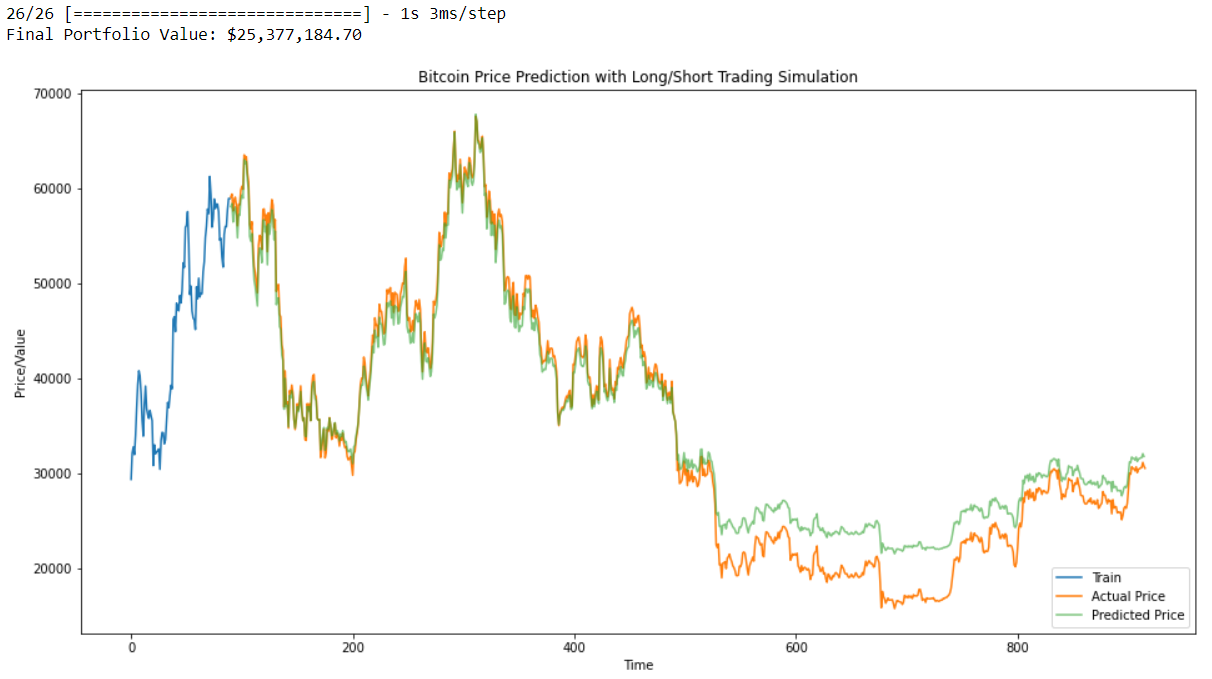
\includegraphics[scale=0.65]{fig13.jpg}
\caption{Adjust the number of days for training(90 Days)}
\label{Adjust the number of days for training}
\end{figure}

Below Visualisation is selected in 300 days.

\begin{figure}[H]
\centering
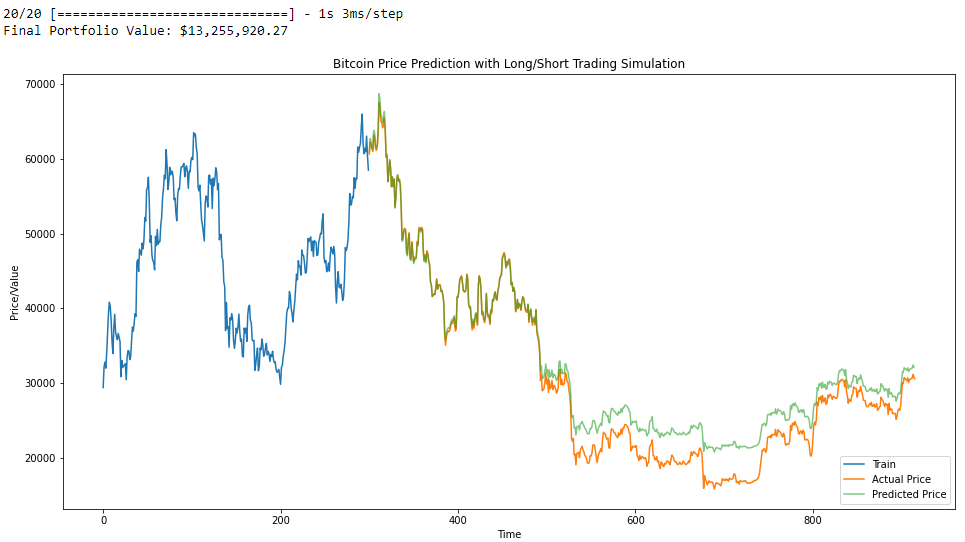
\includegraphics[scale=0.65]{fig14.jpg}
\caption{Adjust the number of days for training(300 Days)}
\label{Adjust the number of days for training}
\end{figure}



\subsection{Conclusion for LSTM Performance:}

The LSTM model has demonstrated its effectiveness in predicting changes in the price of Bitcoin. The model's flexibility when applied to various training window widths and the significant profits made, particularly with a 90 percent training window, highlight its promise for financial forecasting. However, because cryptocurrency markets are inherently unpredictable, it is important to utilize this model's predictions carefully, as with all others.

\section{Comparative Analysis:}

This study conducted a comparative examination of two well-known models, the Random Forest, and the LSTM neural network, in order to gauge the effectiveness of machine learning models in forecasting changes in the price of bitcoin.

\textbf{1.	Model complexity and training time:}

-	 \textbf{Random Forest:} It is a multi-decision tree ensemble learning technique with a relatively complex structure. In contrast to deep learning models, nevertheless, its parallel processing power frequently leads to shorter training times.

-	\textbf{LSTM:} Due to their numerous layers and recurrent structure, LSTM networks are typically computationally demanding. Particularly with larger datasets, they typically take longer to train.

\textbf{2.	Feature Interpretability:}

-	\textbf{Random Forest:} The capability of Random Forest to rate the importance of traits is one of its strengths. This can help with model interpretation and future feature engineering by revealing which features (or variables) are responsible for the predictions.

-	\textbf{LSTM:} Because they are a particular kind of neural network, LSTMs do not naturally provide the same level of feature interpretability as Random Forest. Although there are ways to analyze deep learning models, they are frequently more complicated and might not offer as many insightful details.

\textbf{3. Performance Metrics:}

-	\textbf{ Random Forest:} model demonstrated admirable performance metrics over a range of training and validation periods. It regularly made money and displayed flexibility across various data segments.

-	\textbf{LSTM:} The LSTM model produced a sizable return, especially when trained with a 90 percent window size, demonstrating its promise for financial forecasting. However, with various hyperparameter values or training methods, its performance could vary more noticeably.

\textbf{4.	Economic Implications: }

-   \textbf{Random Forest:} The model's forecasts were translated into a trading strategy that produced large gains, highlighting the model's usefulness for Bitcoin trading.

-   \textbf{LSTM:} The "long or short" trading strategy based on LSTM's predictions on the test data also generated significant gains, highlighting the importance of LSTM from an economic standpoint for Bitcoin trading.

\textbf{5.	Adaptability to New Data:}

-	\textbf{Random Forest:} Even though Random Forest can, in some cases, adapt to changes in data distribution, it may occasionally need retraining or fine-tuning, particularly in extremely volatile markets like cryptocurrency.

-	\textbf{LSTM:} LSTM networks may be better equipped to adapt to the changing nature of financial data because they are built to capture long-term dependencies in sequences. However, in order for them to efficiently recognize new patterns, they may also need retraining on occasion.

\subsection{Conclusion for Comparative Analysis:}

Both the Random Forest and LSTM models have demonstrated their abilities to forecast the course of the Bitcoin price. Long-term temporal patterns are better captured by LSTM networks than by Random Forest, which also may offer faster training times. The decision between the two should take into account the task's specific needs, the computational resources at hand, and how much weight is given to model interpretability. Both models have demonstrated their value in the context of this study, each providing particular advantages in the field of cryptocurrency price prediction.

\section{Summary of the Results}

In this chapter, We looked closely at the outcomes of using the two cutting-edge machine learning algorithms Random Forest and LSTM to forecast changes in the price of bitcoin. The outcomes offer a thorough grasp of the possibilities and capabilities of these models in the complex and unpredictable realm of bitcoin trading. Here is a brief summary:

\textbf{1.	Random Forest Performance:}

-	Time Series Cross-Validation (TSCV) was used to test the ensemble model, which is known for combining several decision trees, throughout a range of training-validation windows.

-	Using performance indicators like RMSE, Accuracy, Precision, Recall, and F1-Score, it was possible to see how well it performed across various data segments in terms of prediction.

-	The significant profits made after turning the Random Forest model's forecasts into a workable trading strategy served to highlight the model's economic importance.

\textbf{2.	LSTM Performance:}

-	The sequential character of the Bitcoin prices was captured using the LSTM, a sort of recurrent neural network.

-	To determine the ideal window size, the model was trained on historical data of varied lengths. The model's capacity to predict prices in light of the quantity of previous data to which it was exposed improved with each iteration.

-	The LSTM model's predictions were translated to a "long or short" trading strategy, similar to the Random Forest model, and the economic results were evaluated.

\textbf{3.	Comparative Analysis:}

-	The two models were compared side by side to reveal their advantages and shortcomings.

-	Model complexity, training time, interpretability of features, performance measures, economic ramifications, and adaptability to new data were some of the factors covered, giving a comprehensive overview of how they apply to cryptocurrencies.

In essence, this chapter emphasizes how machine learning and deep learning models have the ability to make sense of the frequently unexpected world of Bitcoin values. While both models demonstrated admirable performance, they each have distinct advantages, highlighting the need to match the model chosen to the particulars of the forecasting task and the particulars of the available data.


\def\baselinestretch{1.66}
\medskip

%%% ----------------------------------------------------------------------